\documentclass[11pt,a4paper]{article}
\usepackage[margin=2.6cm]{geometry}
\usepackage[T1]{fontenc}
\usepackage[utf8]{inputenc}
\usepackage{booktabs}
\usepackage[hidelinks]{hyperref}
% Let long URLs break across lines; without this the repository URL in
% the Availability section overflows the text block by ~21pt.
\usepackage{xurl}
\hypersetup{
  pdftitle={edikit: A Python Toolkit for Reproducible Construction and
            Auditing of National Social Accounting Matrices},
  pdfauthor={Kodzovi Abalo},
  pdfsubject={Reproducible construction and auditing of national social
              accounting matrices from official statistics},
  pdfkeywords={social accounting matrix; supply and use tables; national
               accounts; reproducibility; RAS balancing; GRAS; data
               provenance; Eurostat; Python}
}
\usepackage[round,numbers]{natbib}
\renewcommand{\bibnumfmt}[1]{#1.}
\usepackage{setspace}
\usepackage{tabularx}
\usepackage{tikz}
\usetikzlibrary{positioning,arrows.meta}
% Expanded acronyms add long unbreakable tokens (European System of
% Accounts (ESA~2010), input--output, CC~BY~4.0) to a 2.6cm-margin
% measure. Allow the last resort a little extra stretch so such lines
% loosen slightly instead of overflowing into the margin.
\emergencystretch=1em
\onehalfspacing

% Drafted in the standard software-metapaper structure (Overview /
% Availability / Reuse potential); to be transferred to the target
% journal's own template at submission.

\title{edikit: A Python Toolkit for Reproducible Construction and
Auditing of National Social Accounting Matrices}
\author{Kodzovi Abalo\\
\normalsize World Bank\\
\normalsize ORCID 0000-0002-7567-2181}
\date{}

\begin{document}
\maketitle

\begin{abstract}
\noindent
\texttt{edikit} is a small Python library for building and auditing
national social accounting matrices (SAMs) from official statistics
under a discipline not yet systematically embedded in commonly
distributed SAM construction workflows: accounting identities are
enforced as executable checks at ingestion and at subsequent pipeline
boundaries, classification is never
inferred silently from labels or code conventions, every balancing
adjustment is logged at
the cell where it acts, and every run writes a validation report that
constitutes the record. The toolkit was developed and validated across five
countries and three exercise types. A cell-level reconstruction and
audit of the published 2019 South African SAM reproduced the production
and commodity structure exactly across all 61 activities and every
final-demand category, and a structure-and-macro-controls audit covered
the IFPRI 2019 Kenya SAM. Benchmark-free generation then produced
balanced macro SAMs for the Netherlands, Austria, and Poland from the
Eurostat dissemination API---three HTTP requests per country, one
command, with confidentiality suppression detected and quantified where
present. Users enter through three documented recipes---replicate,
audit, and build---and the package has one required external
dependency, \texttt{openpyxl}.
\end{abstract}

\vspace{0.5em}
\noindent\textbf{Keywords:} social accounting matrix; supply and use
tables; national accounts; reproducibility; RAS balancing; data
provenance; Eurostat; Python.

\section{Overview}

\subsection{Introduction}

A social accounting matrix (SAM) is a square table recording, for one
economy and one year, every payment made from one account to another.
Rows and columns carry the same ordered list of accounts: activities
that produce, commodities that are produced, factors of production such
as labour and capital, and institutions such as households,
corporations, and government, together with capital accumulation and the
rest of the world. The cell in row $i$, column $j$ holds the payment
from account $j$ to account $i$, so reading along a row gives an
account's receipts and reading down a column gives its outlays. The
defining property is that the two must agree: for every account, total
receipts equal total payments, because every payment is someone else's
income. A SAM is therefore not a collection of statistics but a closed,
internally consistent picture of an economy, and that identity is what
makes it one. National SAMs range from a few dozen accounts to several
hundred.

The matrix is a database, not a model, and it is the empirical
foundation for most applied economy-wide policy analysis. Multiplier
analysis traces how a change in demand propagates through the structure
it records; computable general equilibrium models use it as their
benchmark dataset, calibrating parameters so the model reproduces the
SAM in its base year before any policy is simulated. Ministries of
finance, central banks, development banks, and research institutes rely
on that chain when assessing a tax reform, a tariff change, or a
public-investment programme. Because the model inherits whatever the
matrix contains, an error in a cell does not announce itself: it
propagates silently into results that are read as policy advice.

Building one is a data-reconciliation exercise rather than a modelling
one. The inputs are official statistics---supply and use tables (SUTs),
national and sector accounts, balance-of-payments statistics, household
and labour force surveys---each published on its own classification, in
its own units, at its own vintage, and covering only part of what the
matrix needs. The compiler maps every source category onto the SAM's
account list, fills the cells no source reports, and adjudicates between
sources that measure the same flow and disagree. The assembled matrix
then does not balance, because independent sources were never going to
satisfy the identity by construction, so a final step adjusts cells
until receipts equal payments everywhere---conventionally by the
biproportional method known as RAS, a conventional name rather than an
abbreviation, or by a cross-entropy variant. In practice this is done in
spreadsheets, by one or a few specialists, over weeks or months, and the
judgments made along the way are recorded---when they are recorded at
all---in a prose technical note issued with the matrix. The published
artefact is the matrix and the note; the path from source to cell is not
part of it.

That last gap is what this software addresses. Because the
reconciliation is artisanal and its decisions are documented at best in
prose, published SAMs can seldom be reproduced,
audited, or updated by anyone other than their authors. The companion
methods paper \cite{abalo2026} develops this diagnosis through a
detailed cell-level replication audit of the unusually well documented
2019 South African SAM of van Seventer and Davies
\cite{vanseventer2023}, published by the United Nations University World
Institute for Development Economics Research (UNU-WIDER), and
proposes a remedy: cell-level provenance and machine-readable
construction rules published alongside every SAM. \texttt{edikit} is the
reference implementation of that proposal, released so that the remedy
is a working artefact rather than an exhortation.

The toolkit's design reduces to four commitments. Every source file is
registered with vintage and hash before use. Accounting identities---for
each product, supply at purchasers' prices equals basic-price supply
plus taxes plus margins; for each industry, output equals intermediates
plus value added; for the matrix, every account's receipts equal its
payments---are enforced as executable checks the moment data are read,
not asserted afterwards. Classification is always explicit: account
codes, labels, and header positions are treated as claims to verify,
because the audit found them wrong in even the best-documented matrix in
its class. And adjustment is never silent: the balancing routine returns
the multiplicative factor of every cell it touches, and refuses inputs
it cannot handle transparently.

Existing open tooling in the input--output ecosystem concentrates
primarily on consuming and analysing completed input--output (IO) and
multi-regional input--output (MRIO)
databases---\texttt{pymrio} \cite{stadler2021} is the leading
example, providing parsers, standardisation, and footprint analytics
over compiled databases such as EXIOBASE and the World Input--Output
Database (WIOD). \texttt{edikit}
addresses an earlier, complementary stage of the pipeline: an integrated
workflow for \emph{constructing and auditing} a national SAM against
its underlying official sources. Its distinguishing features are not new
SAM mathematics---RAS, concordances, and the accounting identities are
long established---but the integration of executable accounting checks
at ingestion, explicit and complete account mappings, source-level
provenance, and cell-specific diagnostics for every balancing
adjustment into one testable source-to-artefact workflow.

\subsection{Implementation and Architecture}

Figure~\ref{fig:arch} shows the workflow the library implements; the
same stages serve construction and audit, an audit adding a comparison
target at the reconciliation stage.

\begin{figure}[t]
\centering
\resizebox{\textwidth}{!}{%
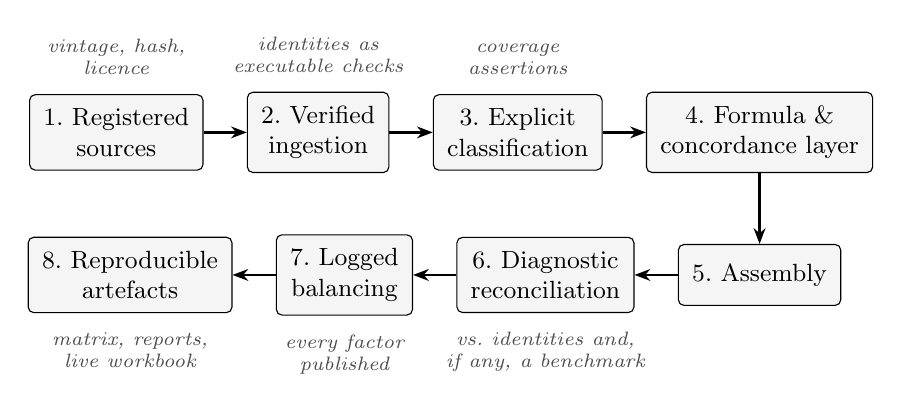
\begin{tikzpicture}[
  stage/.style={draw, rounded corners=2pt, align=center, font=\small,
                minimum height=2.2em, inner sep=5pt, fill=gray!8},
  note/.style={font=\scriptsize\itshape, text=gray!60!black, align=center},
  arr/.style={-{Stealth[length=2mm]}, thick}]
\node[stage] (s1) {1.~Registered\\sources};
\node[stage, right=0.55cm of s1] (s2) {2.~Verified\\ingestion};
\node[stage, right=0.55cm of s2] (s3) {3.~Explicit\\classification};
\node[stage, right=0.55cm of s3] (s4) {4.~Formula \&\\concordance layer};
\node[stage, below=0.9cm of s4] (s5) {5.~Assembly};
\node[stage, left=0.55cm of s5] (s6) {6.~Diagnostic\\reconciliation};
\node[stage, left=0.55cm of s6] (s7) {7.~Logged\\balancing};
\node[stage, left=0.55cm of s7] (s8) {8.~Reproducible\\artefacts};
\draw[arr] (s1) -- (s2); \draw[arr] (s2) -- (s3);
\draw[arr] (s3) -- (s4); \draw[arr] (s4) -- (s5);
\draw[arr] (s5) -- (s6); \draw[arr] (s6) -- (s7); \draw[arr] (s7) -- (s8);
\node[note, above=0.12cm of s1] {vintage, hash,\\licence};
\node[note, above=0.12cm of s2] {identities as\\executable checks};
\node[note, above=0.12cm of s3] {coverage\\assertions};
\node[note, below=0.12cm of s6] {vs.\ identities and,\\if any, a benchmark};
\node[note, below=0.12cm of s7] {every factor\\published};
\node[note, below=0.12cm of s8] {matrix, reports,\\live workbook};
\end{tikzpicture}%
}
\caption{The workflow \texttt{edikit} implements, from registered
sources to reproducible artefacts.}
\label{fig:arch}
\end{figure}

\texttt{edikit} is pure Python (about 1{,}500 lines in the implemented
core), organised in four modules with one external dependency
(\texttt{openpyxl}, for Excel I/O):

\begin{itemize}
  \item \texttt{edikit.data} --- readers for the source families a SAM
  build encounters: SUT workbooks (recomputing every embedded
  total and enforcing the layout's identities), distributed SAM
  matrices, central-bank time-series bulk files with a small evaluator
  for signed series formulas, Eurostat JSON-stat responses (decoding the
  dissemination API's linear index into code-keyed cells), and
  concordances with completeness validation.
  \item \texttt{edikit.model} --- the account taxonomy with coverage
  assertions (every account classified, nothing phantom; classification
  is never inferred silently from labels or code conventions---any
  prefix rules must be explicitly declared, reviewable, and complete,
  and unmatched accounts raise), together with RAS and generalised RAS
  (GRAS) balancing. RAS requires
  a non-negative seed, verifies target consistency, reports convergence,
  and returns per-cell adjustment factors as a first-class result; GRAS
  admits negative entries.
  \item \texttt{edikit.report} --- generation of Excel workbooks whose
  totals and balance checks are live formulas rather than pasted
  numbers, so a reader can interrogate the artefact in the tool they
  already use.
  \item \texttt{edikit.pipeline} --- end-to-end routines:
  \texttt{eurostat\_sam} (fetch, generate, balance, and report a macro
  SAM for countries the European System of Accounts (ESA~2010)
  transmission datasets cover, including
  coverage-based classification-tiling assertions and
  suppressed-detail handling) and \texttt{audit} (structural audit of
  any distributed SAM, plus macro-aggregate comparison against published
  national-accounts controls).
\end{itemize}

Table~\ref{tab:modules} lists the principal public entry points.

\begin{table}[h]
\centering\small
\begin{tabularx}{\textwidth}{llX}
\toprule
Module & Key callables & Role \\
\midrule
\texttt{data.sut} & \texttt{read\_supply\_table}, \texttt{read\_use\_table} & SUT ingestion with identity checks \\
\texttt{data.sam} & \texttt{read\_labeled\_matrix} & distributed SAM workbooks \\
\texttt{data.kbp} & \texttt{read\_kbp\_zips}, \texttt{evaluate\_formula} & central-bank series and signed formulas \\
\texttt{data.eurostat} & \texttt{read\_jsonstat}, \texttt{EurostatTable} & dissemination-API responses \\
\texttt{data.concordance} & \texttt{Concordance} & mappings with completeness validation \\
\texttt{model.accounts} & \texttt{AccountSet}, \texttt{AccountKind} & explicit taxonomy, coverage assertions \\
\texttt{model.balancing} & \texttt{ras}, \texttt{gras}, \texttt{BalanceResult} & RAS and GRAS with per-cell factor diagnostics \\
\texttt{report.workbook} & \texttt{add\_matrix\_sheet}, \texttt{add\_table\_sheet} & live-formula Excel artefacts \\
\texttt{pipeline.eurostat\_sam} & \texttt{fetch}, \texttt{generate}, \texttt{balance} & macro-SAM generation (ESA countries) \\
\texttt{pipeline.audit} & \texttt{audit}, \texttt{read\_kinds} & structural and macro-controls auditing \\
\bottomrule
\end{tabularx}
\caption{Principal public entry points by module.}
\label{tab:modules}
\end{table}

Users enter through three documented \emph{recipes}, thin scripts over
the library: \texttt{replicate/} regenerates every number in the
companion paper; \texttt{audit/} audits a published SAM
(\texttt{python audit\_sam.py -{}-sam matrix.csv -{}-kinds kinds.csv
-{}-controls controls.csv}); \texttt{build/} generates and balances a
macro SAM for a country-year (\texttt{python build\_sam.py -{}-country
AT -{}-year 2019}). Every pipeline run writes a markdown validation report
recording each identity check, coverage diagnostic, and account
residual, and---when balancing is invoked---convergence, flipped cells,
and the adjustment-factor range, with the factor of every individual
cell in the balanced CSV; the reports, not the console, are the
record. The
recipes are thin by design: the same functionality is available through
a short library workflow, for example:

{\small
\begin{verbatim}
from edikit.pipeline import eurostat_sam as es

paths = es.fetch("AT", 2019, "data/")     # three cached API requests
res   = es.generate("AT", 2019, paths)    # identities checked; residuals attributed
bal, flipped = es.balance(res)            # RAS; every factor in bal.factors
es.write_report(res, "AT_2019_generation.md",
                balance=bal, flipped=flipped)
es.write_balanced_csv(bal, "AT_2019_macro_sam_balanced.csv")
\end{verbatim}}

\noindent The Dutch case runs entirely offline from three registered
Eurostat responses committed in the repository, which is the recommended
first run (the repository README's ``reviewer pathway''). Its validation
report reads, in excerpt, with residuals expressed as shares of gross
domestic product (GDP):

{\small
\begin{verbatim}
Output and VA identities: 0 findings at EUR 1m tolerance
Commodity balance closure: 65/65 products within EUR 1m
GDP at basic prices (generated): EUR 724,960m
lab residual: -4,193 EUR m (-0.578% of GDP)
row residual: -10,830 EUR m (-1.494% of GDP)
RAS converged in 418 iterations; max residual EUR 0.009m
Adjustment factors: 70 cells in [0.9832, 1.0282]
\end{verbatim}}

\subsection{Quality Control}

Three layers. First, a \texttt{pytest} suite (38 tests at the tagged
release) in which the accounting identities are the test cases, covering
the readers, the classification and tiling machinery, RAS and GRAS
diagnostics, the audit pipeline, the cross-producer reconciliation
reporter, and end-to-end generation and balancing on a
synthetic two-industry economy whose identities close exactly. Every
test runs from inputs shipped in the archive, so a reviewer working from
the archive or a repository clone sees \texttt{38 passed}. Installing
the package alone from PyPI brings the library and its tests but not the
papers' data directories, so the Kenya integration test skips there. Line
coverage is 93\,per\,cent overall (84--100\,per\,cent per implemented
module; \texttt{pytest toolkit/tests -{}-cov=toolkit/src/edikit}); this
measures which code paths are exercised, while the identity-based and
end-to-end tests carry the evidence of domain correctness. A
continuous-integration workflow runs the suite on Linux, macOS, and
Windows across Python versions 3.11--3.13 on every push. Beyond the five
validation countries, a committed coverage sweep
(\texttt{recipes/build/sweep.py}) runs the build pipeline across 37
candidate countries for 2019 and classifies every outcome on the
toolkit's own terms: 11 pass every core check (zero identity findings,
full commodity closure, no cross-table differences, import identity
within tolerance, no suppression, converged balancing, worst residual
within 5\,per\,cent of GDP); 9 generate and balance with documented
caveats; 7 carry large residuals or extreme factors and require review;
2 generate but cannot be balanced from one-sided sector accounts; and 8
country-years are not covered by the datasets. The archived Zenodo deposit is the snapshot of
the tagged release this paper describes, and the reviewer pathway's
expected console output is stated verbatim in the repository README, so
a successful installation is verifiable in minutes. Second, run-time assertions in every pipeline:
coverage assertions on classification, tiling assertions on
category-list partitions, target-consistency checks in balancing. These
assertions have each caught real errors during development---a survey
parser that silently dropped an industry with 6{,}202 observations, and
a double-count from Eurostat's mixed-granularity category lists---which
the companion paper reports as evidence that the checks bind. Third,
validation at scale across five countries and three exercise types,
summarised in Table~\ref{tab:validation}; each run's full validation
report ships with the repository, and the Polish case demonstrates the
principal failure mode handled transparently---confidentiality
suppression is detected by the tiling assertions, quantified per
aggregate, and reported rather than absorbed.

\begin{table}[t]
\centering\small
\begin{tabularx}{\textwidth}{lXX}
\toprule
Country (2019) & Exercise & Outcome \\
\midrule
South Africa & cell-level reconstruction, audited against the published
UNU-WIDER benchmark & Production and commodity structure exact on all 61
activities and every final-demand category; 43 of 45 computable macro
cells exact. The two exceptions both reflect one unrecorded
R596~million reconciling adjustment applied symmetrically; the
benchmark's single unpublished input was priced separately. \\
Kenya & structural and macro-controls audit of the International Food
Policy Research Institute (IFPRI) Nexus SAM &
structure verified; matrix balanced to its distribution's rounding
grain; production side within 1\% of published controls \\
Netherlands & benchmark-free generation and balancing & zero identity
findings (65/65 industries and products); all residuals attributed,
each $\leq$1.5\% of GDP; balanced to $<$EUR~0.01m at full precision
with factors in $[0.9832, 1.0282]$ \\
Austria & transferability: the same generator rerun unchanged on a new
country & zero identity findings; residuals $\leq$0.6\% of GDP \\
Poland & suppression stress test & withheld cells detected (leaf detail
covers 96.7\% of gross output); macro accounts anchored to published
totals; residuals $\leq$1.1\% of GDP \\
\bottomrule
\end{tabularx}
\caption{Validation across five countries and three exercise types.}
\label{tab:validation}
\end{table}

\section{Availability}

\subsection{Operating system}
Pure Python; the test suite runs in continuous integration on Linux,
macOS, and Windows.

\subsection{Programming language}
Python $\geq$ 3.11.

\subsection{Additional system requirements}
None; memory and disk requirements are trivial (national SUT and
sector-accounts inputs are megabytes).

\subsection{Dependencies}
\texttt{openpyxl}. Optional: \texttt{certifi} (TLS trust store for API
fetches on platforms without system certificates); \texttt{pytest} and
\texttt{pytest-cov} (development).

\subsection{Software location}
\begin{description}
  \item[Package index:] PyPI, \url{https://pypi.org/project/edikit/};
  \texttt{pip install edikit} installs the library and its dependency,
  and a specific release can be pinned in the usual way
  (\texttt{pip install edikit==0.2.5}). The repository remains the route
  for the replication recipes and their registered inputs, which are not
  part of the package.
  \item[Code repository:] GitHub,
  \url{https://github.com/kodzovee9/tekmeris} (toolkit under
  \texttt{toolkit/}); licence Apache-2.0; version 0.2.5, July 2026.
  \item[Archive:] Zenodo, DOI
  \href{https://doi.org/10.5281/zenodo.21477787}{10.5281/zenodo.21477787}
  (version v0.2.5; concept DOI for all versions:
  10.5281/zenodo.21419195); licence Apache-2.0.
\end{description}

\subsection{List of contributors}
Kodzovi Abalo (design, development, validation).

\subsection{Language}
English.

\section{Reuse Potential}

Three reuse paths correspond to the three recipes. Researchers can
generate a validated, balanced macro SAM with one command and no manual
data step for the countries the Eurostat datasets cover---the committed
coverage table documents exactly which: for 2019, 11 of 37 candidates
pass every core accounting check, a further 9 generate and balance with
documented caveats, and every remaining case is classified and
recorded. The same command run across countries gives
comparably constructed matrices with per-country validation reports---including, where publication practice withholds cells, an
explicit statement of what was suppressed. Analysts holding any
distributed SAM can run the structural audit unmodified (two CSV
sidecars---an account-classification table and published controls---
enable the macro comparison), which makes routine due diligence on
third-party SAMs practical for model users who did not build the matrix
they depend on. And compilers working outside the harmonised
universe can adapt the South African pipeline pattern documented in the
recipes: registered sources, identity-checked ingestion, explicit
concordances, formula tables, and logged balancing, reusing the library
wholesale and replacing only country-specific configuration.

Reusers should know the current limitations plainly. Version 0.2.5
implements classical RAS and GRAS \cite{temurshoev2013}---the latter
negative-tolerant, so matrices carrying negative cells can be balanced
directly. Standard RAS requires a non-negative seed. The Eurostat
pipeline applies an explicitly reported sign-normalisation rule to the
limited negative flows it encounters, and refuses inputs it cannot
handle that way; matrices with general negative entries should use GRAS
instead. The toolkit does not implement general cross-entropy balancing
against an arbitrary prior \cite{robinson2001}, which matters most where
margins are partial or additional constraints are imposed. The automatic
Eurostat workflow produces a
macro SAM, not a fully disaggregated multi-sector and household SAM.
Adaptation outside the Eurostat universe requires country-specific
source readers and mappings. Statistical confidentiality can prevent
full cell-level reconstruction---the toolkit detects and quantifies
suppression, but cannot undo it. And an accounting-consistent output is
not necessarily an economically preferred allocation where multiple
admissible mappings exist; the toolkit's contribution is to make the
chosen mapping visible, not to certify it unique.

Natural extensions, deliberately scoped out of version 0.2.5, include
cross-entropy balancing against a prior under partial margin information
\cite{robinson2001}, full multi-sector (rather than
macro) generation from the 65-industry ESA core, and survey-driven
household disaggregation following the companion paper's South African
scripts. User support, bug reports, and feature requests are managed through
the repository's GitHub Issues page; contributions are welcome, and the
test suite and the identity-as-assertion discipline define the contract
new code must meet.

\section*{Data Accessibility Statement}
The versioned software, redistributable sample inputs, validation
reports, and generated outputs are archived on Zenodo at
doi:10.5281/zenodo.21477787. Third-party inputs whose licences do not permit
redistribution are not included; for each restricted input, the
repository's \texttt{SOURCES.md} records the publisher, source
location, access date, licence or access conditions, and SHA-256
checksum required to verify a locally obtained copy.

\section*{Generative AI Use}
Generative AI (Anthropic's Claude) was used for code generation and
diagnosis. All generated code,
mappings, and outputs were reviewed by the author and accepted only
after the deterministic accounting checks and tests described above
were satisfied. The author assumes full responsibility for the
software.

\section*{Author Roles}
Kodzovi Abalo: conceptualisation, software design and development,
validation, writing.

\section*{Acknowledgements}
The toolkit's validation relied on data published or distributed by
Statistics South Africa, the South African Reserve Bank, the Kenya
National Bureau of Statistics, IFPRI, UNU-WIDER, and Eurostat; the
unusually thorough documentation of the UNU-WIDER 2019 South African SAM
\cite{vanseventer2023} is what made cell-level validation possible.

\section*{Disclaimer}
The views expressed here are those of the author and do not necessarily
reflect the views of the World Bank, its Executive Directors, or the
governments they represent.

\section*{Funding Statement}
No dedicated funding was received for the development of the software or
the preparation of this manuscript.

\section*{Competing Interests}
The author declares no competing interests.

\section*{Copyright and Licence}
This paper is released under a Creative Commons Attribution 4.0
International licence (CC~BY~4.0): it may be copied, redistributed, and
built upon for any purpose, including commercially, provided attribution
is given. The software it describes is released separately under the
Apache-2.0 licence, as recorded under Software location above. Neither
grant extends to third-party inputs, which keep the terms recorded for
each of them in the repository's \texttt{SOURCES.md}.

\bibliographystyle{vancouver}
\bibliography{references}

\end{document}
